
\documentclass[a4paper,11pt]{article}

\usepackage{amsmath,amssymb,amsfonts,amsthm}    % Typical maths resource packages
\usepackage{graphicx}                           % Packages to allow inclusion of graphics
\usepackage{hyperref}                           % For creating hyperlinks in cross references
% \usepackage[authoryear]{natbib}                 % literature reference style
\usepackage[bf]{caption}

% Biblatex
\usepackage[english]{babel}
% \usepackage{csquotes}
\usepackage[style=authoryear]{biblatex}
\addbibresource{../content/refs/references.bib}% Syntax for version >= 1.2

% -------------------------------
% --- some layout definitions ---
% -------------------------------

% define topline
\usepackage[automark]{scrlayer-scrpage}
\pagestyle{scrheadings}
\automark{section}
\clearpairofpagestyles
\ohead{\headmark}

% define citation style
% \bibliographystyle{plainnat}

% define page size, margin size
\setlength{\headheight}{1.1\baselineskip}
\voffset=-2cm
\hoffset=-3cm
\textheight24cm
\textwidth15.5cm
\topmargin1cm
\oddsidemargin3cm
\evensidemargin3cm

% define line line spacing = 1.5
\renewcommand{\baselinestretch}{1.5}

% define second level for `itemizing'
\renewcommand{\labelitemii}{-}

\begin{document}

% -------------------------------
% --- frontmatter: Title page ---
% -------------------------------

\thispagestyle{empty}
\begin{center}

    {\Large{\bf Causal Forests}} \vspace{0.5cm}

    {\large{\bf How machine learning can enhance econometrics in uncovering heterogeneous causal effects.}} \vspace{0.5cm}

    {\normalsize Seminar New Models for the Digital Economy\\\vspace{0.5cm}}
    {\normalsize{\bf Prof. Michael Burda, PhD}} \\\vspace{0.5cm}
    {\normalsize Humboldt-Universit\"at zu Berlin \\
    School of Business and Economics \\
    % Institute for Statistics and Econometrics \\
    Institute for Economic Theory II} \vspace{1cm}

    {\normalsize by \\\vspace{0.5cm}
    {\bf Denis Augusto Pinto Maciel} \\
    (505471)} \vspace{1cm}


    {\normalsize Berlin, July 20, 2019}

\end{center}


% ------------------------------------
% --- frontmatter: Acknowledgement ---
% ------------------------------------
% \newpage
% \pagestyle{plain}
% \pagenumbering{roman}   % define page number in roman style
% \setcounter{page}{1}    % start page numbering
% \input{../content/fix/acknowledgement}

% -----------------------------
% --- frontmatter: Abstract ---
% -----------------------------
\newpage
% \input{../content/fix/abstract}

% -----------------------------
% --- frontmatter: Contents ---
% -----------------------------
\newpage
\tableofcontents
\clearpage

% % ----------------------------------------------------
% % --- frontmatter: List of Abreviations (not mandatory) ---
% % ----------------------------------------------------
% \newpage
% \addcontentsline{toc}{section}{List of Abbreviations}
% \ohead[]{LIST OF ABBREVIATIONS}
% \input{../content/fix/abbreviations}

% % ----------------------------------------------------
% % --- frontmatter: List of Figures (not mandatory) ---
% % ----------------------------------------------------
% \newpage
% \addcontentsline{toc}{section}{List of Figures}
% \ohead[]{\rightmark}
% \listoffigures


% % ---------------------------------------------------
% % --- frontmatter: List of Tables (not mandatory) ---
% % ---------------------------------------------------
% \newpage
% \addcontentsline{toc}{section}{List of Tables}
% \listoftables


% -------------------------------
% --- main body of the thesis ---
% -------------------------------
\newpage
\pagestyle{plain}
\setcounter{page}{1}    % start page numbering anew
\pagenumbering{arabic}  % page numbers in arabic style


\section{Introduction}

% Prediction vs Causality
Economists are faced with two related, but very different type of questions. There is the question about prediction and there is the question about causality. This duality can be better illustrated by an example: the demand for hotel rooms. If we were given past data on room prices and occupancy of hotels, we would encounter a positive correlation between them: whenever the price is high, occupancy is expected to be high as well. Knowing nothing else, if you were asked to predict the price of a hotel whose occupancy is high, you should predict the price to be high as well. A naïve hotel owner, however, might conclude that by raising prices, he will increase the occupancy of his establishment. This, of course, doesn't make sense in the light of economic theory. The hotel owner is mixing up correlation with causation, prediction with causality. Demand for a good decreases as its price goes up. In the hotel case, there is a third factor that drives both demand and prices up. Vacation season increases demand for hotel rooms. Seeing this, hotel owners by raising prices. Thus, it becomes clear that the surge in demand due to high season is strong enough to make occupancy increase \textit{despite} the simultaneous price increase.

The search for causality has been long one of the main concerns of economists. In recent years, machine learning - a field that has been mostly concerned with prediction - started to be used together with econometrics to answer questions about causal inference. Following these new developments, we will reassess in this paper the question about the causal effect of Medicaid coverage on visits to the emergency department. This problem has been already analyzed with battle-tested econometric methods by \cite{taubmanMedicaidIncreasesEmergencyDepartment2014} . Here, however, we will provide an overview about causal inference, heterogeneitey in causal effects and how decision trees can be stiched together to uncover causal effects. Finally, we will apply causal forests, a method whose basic structure was developed within machine learning (\cite{breimanRandomForests2001}), to try to identify heterogeneity in the response to Medicaid coverage.


% Econometrics we will be analyzing a Machine learning and econometrics approach their fundamental questions they are trying to answer in different ways. At the heart of econometrics lies the constant search for an explanation. Econometricians won't think twice before sacrificing goodness of fit of their models to achieve a better, more precise estimate of the parameter whose ground truth they are trying to uncover. Machine learning focuses rather on prediction. It has developed during the last decades various techniques, heuristics and methods that have made it very successful in different fields.

\newpage

\section{Causality \& Experiments}

Does Medicaid\footnote{Although frequently mentioned together in the media, Medicaid and Medicare are two separate programs. Medicare is a federal program that provides health coverage for adults ages 65+ and disabled people irrespective of their incomes. Medicare is both sate and federal and provides health coverage for low-income adults.} coverage increase or decrease the number of visits of a person to the emergency department? This question comes up whenever an expansion of Medicaid is considered. This is the case mostly because of the fiscal impact that an increase or decrease of emergency department visits resulting from more people having access to Medicaid could have. There are two lines of reasoning about what could be the effect of a Medicaid expansion on the state of public finance. The first one argues that by granting insurance to more people, one is to expect an overall higher usage of health care and thus an increase in public spending. A second line of reasoning defends that a Medicaid expansion could decrease insurance spending. Medicaid would allow participants to have greater access to primary care and by doing so it would be able to prevent acute conditions that result in an emergency department visit. Emergency department visits, it turns out, are much more costly than primary care. According to this line of reasoning, access to Medicaid and the ensuing increase in primary care (which is cheaper) would reduce the usage of emergency departments (which is considerably more expensive). This way, Medicaid would end up having a positive effect on public accounts.

\subsection{The Oregon Health Insurance Experiment}

In 2008, the state of Oregon opened a waiting list for the expansion of Medicaid. The program had been closed for new enrollments for over four years. As detailed in \cite{finkelsteinOregonHealthInsurance2012}, the expansion targeted low-income adults that would otherwise not be eligible for Medicaid. More specifically, those eligible for the program were adults ages 19-64 who were Oregon residents, either U.S. citizens or legal immigrants, have not had health insurance for the past six months, had income below the federal poverty level and had assets below \$2,000. There were 10,000 available slots.

Oregon has correctly anticipated the high demand for the program and decided to run a lottery to pick the winners. This is the perfect scenario for identifying and disentangling causal effects of Medicaid. As explained below, the randomization in treatment assignment coming from the lottery draws enable us to isolate the effect of treatment from other otherwise correlated covariates.

Registration for the lottery was available for one month from January 28 to February 29, 2008. The state went on to publicize the lottery and the barriers to sign-up were relatively low: anyone could sign-up by telephone, by fax, by mail, in person or online. At the end of the five-week window, 89,824 individuals were registered in the lottery list. During the following months (March through September 2008), the state conducted eight lottery drawings. In each one of them, roughly the same number of participants were selected. As soon as an individual was selected, all members of her household became eligible for entering Medicaid. 35,169 individuals from 29,664 different households were selected by lottery. About 30\% of the selected individuals ended up successfully enrolling in the program. Only 60\% of the selected individuals sent an application and from the applications sent, about half of them were deemed ineligible.

The data used in our paper was made available by \cite{finkelsteinOregonHealthInsurance2012} and can be downloaded at \url{https://www.nber.org/oregon/4.data.html}.

\subsection{Why experiments work?}

In an ideal world (with observable parallel universes), the causal effect of Medicaid coverage on emergency department visits could be estimated for every single individual by subtracting the number of visits under Medicaid from the number of visits without Medicaid that he or she had. For obvious reasons, a person can either be under treatment or control. We can never observe both states of the world simultaneously. The impossibility to observe the same person under treatment and control has come to be known as the \textit{fundamental problem of causal inference}.

Instead of individual treatment effects, an alternative is to try to estimate the \textit{average} treatment effect of a population (\cite{morganCounterfactualsCausalInference2015}). To make what follows understandable, it's important to first define some basic notation:

\begin{itemize}
  \item $Y_0$: dependent variable $Y$ when under control
  \item $Y_1$: dependent variable $Y$ when under treatment
  \item $T \in \{0,1\}$: dummy varible indicating whether observation is under treatment or control
  \item $\pi$: share of population under treatment
\end{itemize}

With that in mind, the average treatment effect can be defined as:

\begin{equation}
  ATE = \mathbb{E}[Y_1 - Y_0] = \mathbb{E}[Y_1] - \mathbb{E}[Y_0]
\end{equation}

By taking into account the actual treatment taken by each share of the population, we can rewrite the equation above as:

\begin{equation}
  \label{eq:ate_decomposed}
    ATE = \{\pi \mathbb{E}[Y_1 | T = 1] + (1-\pi) \mathbb{E}[Y_1 | T = 0]\} \\
    - \{\pi \mathbb{E}[Y_0 | T = 1] + (1-\pi) \mathbb{E}[Y_0 | T = 0]\}
\end{equation}

Formulating the problem in terms of average treatment effects does not by itself free us from the fact that some states are unobservable. In equation \ref{eq:ate_decomposed}, the expected value of $Y_1$ for the share of population under control  ($\mathbb{E}[Y_1 | T = 0]$)  and the expected value of $Y_0$ for the share of population under treatment (($\mathbb{E}[Y_0 | T = 1]$)) cannot be observed. In general, groups under treatment and control are different and have, for this reason, different expected values of the dependent variable. For example, in the absence of an experiment setting, a group of people taking a new drug with unknown side-effects (treatment) is in all likelihood very different from those not taking it (control). Those taking the drug could be much sicker than those not taking it and, therefore, willing to take higher risks to achieve a potential cure. In this scenario, comparing the average health (the dependent variable) of treatment and control wouldn't make sense, since those in treatment have already worse health and, even if the drug has a beneficial effect, treatment's average health would still be lower than control's.

This, however, wouldn't be a problem if we knew exactly which variables are responsible for the differences in treatment and control. We could simply control for them (i.e., include them in the regression as dependent variables) and our estimates of treatment effects would be accurate. Yet not only can we not be sure about all variables that drive differences in treatment and control groups, but also some of these variables are not observable in the first place. Going back to Medicaid and emergency department case, it's plausible that the psychological traits of individuals do play a role in the number of visits to the emergency department they have. A person can have many visits to the emergency department either because she is truly sick or because she has a more cautious personality. Although her health condition is observable (we can measure her blood pressure and glucose levels, etc), the psychological condition of someone being overly cautious and visiting the emergency department at the first suspicion of illness is not. Unobservable variables cannot, per definition, be controlled for making it impossible in an observational study to disentangle its effects from the variable we are trying to analyze. In such situations trying to estimate the effect of Medicaid on emergency department visits will probably be affected by omitted variable bias. Specifically, since we expect overly cautious people to be already in Medicaid, we would estimate that the effect of Medicaid on increasing emergency department visits is higher than what it is in fact.

Random assignment of treatment frees us from the two problems mentioned above. By randomly selecting participants to receive the treatment, we expect treatment and control groups to be equal in every single aspect except for the treatment variable. Thus, any difference arising between the two groups must be caused by the variable whose causal effect we are trying to estimate. On the one hand, we can estimate average treatment effects directly by computing $ATE = \mathbb{E}[Y_1 | T = 1] - \mathbb{E}[Y_0 | T = 0]$, since $\mathbb{E}[Y_1 | T = 1] = \mathbb{E}[Y_1 | T = 0]$ and $\mathbb{E}[Y_0 | T = 1] = \mathbb{E}[Y_0 | T = 0]$. On the other hand, random assignment breaks the correlations between unobservable variables and our treatment, because the latter was randomly assigned.

The subjects of the Oregon Health Insurance Experiment (OHIE) were randomly assigned to the treatment (Medicaid). This is a perfect setting for assessing the causal effects that Medicaid might have in other variables. The first step in such an analysis is to make sure that the experiment was able to balace control and treatment groups. For that, we compare both groups with respect to the variables we can observe.  In OHIE, we compared mean year of birth, percentage of female, percentage that provided a phone number, percentage that signed up for lottery list on the first day across treatment and control. Table \ref{tab:treatment_control_comparison} shows that the difference between treatment and control across all metrics are very small and none is significantly different from zero. This is indicative that the lottery has managed to create comparable groups and that any significant variation in emergency department visits can be attributed to access to Medicaid or lack thereof.

\begin{table}[ht]
\centering
\begin{tabular}{rlrrr}
  \hline
    & Metric & Control Average & Treatment Average &  Difference \\ 
  \hline
   & year\_of\_birth          & 1968.34 & 1968.50 &  -0.16 (0.21)\\ 
   & pp\_female (\%)          & 55    & 54        &  1.1 (0.7) \\ 
   & gave\_phone\_number (\%) & 87    & 88        &  -1.0 (0.8) \\ 
   & first\_day\_list (\%)    & 9     & 10        &  1.0  (0.7)\\ 
   \hline
\end{tabular}
   \caption{\label{tab:treatment_control_comparison} Comparison between groups under treatment and control}
\end{table}

\newpage

\section{Heterogeneity in Treatment Effects}

Heterogeneous treatment effect is a mouthful, but ultimately a very simple concept. It refers to the fact that different people might react differently to the same treatment. Take the fictional example of a \$1000 transfer to individuals from a specific population. This is our treatment. Imagine there are two groups in our population: drug addicts and non-drug addicts. We want to measure the impact that this transfer has on the health of the individuals. Here we measure health with an index that ranges from 0 to 100. In this fictional example, \$1000 cause the health of drug addicts to decrease because they will use the money to acquire more drugs. For non-drug addicts, the effect on health is positive. 

\begin{table}[h!]
  \begin{center}
    \caption{Simple Heterogeneity Example}
    \label{tab:heterogeneity}
    \begin{tabular}{l|r|r|r}
         & \textbf{\$1000} & \textbf{\$0} & \textbf{Treatment Effect}\\
      \hline
        Non drug addicts & 64 & 62 & 2\\
        Drug addicts     & 17 & 25 & -8\\
    \end{tabular}
  \end{center}
\end{table}

If the population is comprised of 95\% of non-drug addicts, the estimate of the average causal effect (ATE) of a \$1000 transfer on health would be of 1.5 points in the health index.

\begin{equation}
    ATE = 2 \times 0.95 + (-8) \times 0.05 = 1.5
\end{equation}

Across the whole population, the average treatment effect is positive, even though for the drug addict group the treatment has a nefarious effect. A well-meaning policymaker would probably want to identify these two groups and target them differently.

% Heterogeneity & Big data

It's easy to see how heterogeneity can take much more complex forms. We need not stop in differences across two groups, we can think as many groups as there are characteristics identifying the units of observation. In the specfic case, one could think of age, gender, and marital status as also influencing the response of the individuals to treatment.

Researchers haven't been blinded to heterogeneity in causal effects. On the contrary, many methods, very complex and otherwise, have been developed to disentangle different groups with different reactions to treatment (\cite{imbensIdentificationEstimationLocal1994}). Usually, the identification and estimation of treatment effects take the form of a specification plan done before the data collection where the researcher determines which covariates she suspects may be a source of heterogeneity. The pre-specification aims to refrain researchers from cherry-picking covariates after data collection that seems a statistically significant source of heterogeneity. After all, if enough covariates are measured, some combination of them will by chance pass the statistical tests for heterogeneity.

With the rise of big data, however, researchers have been faced with yet a different problem. On the one hand, they want to make use of every piece of information that is relevant for identifying heterogeneous treatment effects. But there is the problem that if one looks long enough, she will find heterogeneity that comes to be due to sampling. The tension between the scientificity of a method and the desire to extract relevant information from the data can be softened with the aid of machine learning.

\newpage

\section{Causal Forest}

\subsection{Decision Trees 101}

Imagine you are in charge of the lending department of a bank. You receive daily many requests of people wanting to borrow money from your employer. Along with those requests, you have access to a myriad of information on each applicant: age, gender, income statement, marital status and so on. You also have the same data on people who have gotten loans in the past. For the past loans, you also know if they have been paid back or the borrower has defaulted. Your task is to decide which of the new applicants should be granted a loan and you should pick ideally only those who won't default should.

One way of doing this is to apply a decision tree. In its most general form, a decision tree is a set of rules that splits a population into smaller groups. In our example, we want to split our applicants into subgroups and for each one of them, we either grant or reject a loan to the applicants belonging to it. The way you come up with rules can be arbitrary. You could probably use common sense and only grant loans to those with income over a certain threshold. In this case, you would end up with a very shallow tree with two leaves (also called end nodes): one leaf would contain those who make more than your threshold and the other one would contain those who make less. Nothing is limiting the number of nodes in your tree. In fact, you could grow your tree to have as many nodes as there are applicants (as long as the information you have on them is enough to uniquely identify each one of them). For example, you could be more restrictive with loan granting and after the split based on income, you further split the node of high-income participants into younger and older than 25. Only those applicants with high income and above 25 years would be granted a loan.

Although decision trees can accommodate a variety of heuristics when building the tree, machine learning practitioners take a more principled approach when deciding which rules to pick in order to split each node. Specifically, they look at past data and try to find rules that nicely splits the dataset according to a metric.\footnote{ Many metrics can be used to quantify prediction error. In regression, the root mean squared error (RMSE), defined by $\sqrt{\frac{\sum_{i = 1}^n ({y_i - \hat{y}_i})^2  }{n}}$, is normally used. In classification, there are various metrics to be chosen from. The choice of a metric is dependent on the nature of the problem. Accuracy (the ratio between the number of correctly predicted classes and the total number of observations) would be a poor choice in the case the task is to identify individuals with a rare disease.} Here, we would look at data on past loans and try to minimize the number of defaults, while still granting loans to solvent applicants. To make matters simple, let's assume that to grant a loan to a defaulting applicant is as costly as rejecting a loan to a creditworthy applicant (i.e. a false positive is equivalent to a false negative in terms of cost). With this assumption in mind, we can use as our metric the accuracy, the ratio between the number of correctly identified applicants and the total number of applicants.

Finally, we need a loss function. Something that our algorithm will try to minimize as the ultimate criteria when picking splitting rules. For classification tasks, it's usual to pick entropy. In classification with $n$ classes, the entropy $H$ for every node $S$ in a tree is defined as

\begin{equation}
    H(S) = \sum_{i = 1}^n{-p_i \ln p_i}
\end{equation}

where $p_i$ is the proportion of class $i$ present in node $S$.

In our two-class example, the entropy in each leaf boils down to $H(S) = - p_{c}  \ln p_{c} - p_{d} \ln p_{d}$. Figure \ref{fig:entropy} illustrates how entropy in a node varies in a two-class scenario with the proportion of one of the classes. Node entropy is the total entropy in the node, while partial entropy shows only the contribution of one of the classes to total entropy. To minimize entropy, our algorithm must create splits with as many applicants of one type as possible. The entropy is minimized when the share of creditworthy applicants is either zero or one. In other words, the entropy at a certain leaf will be zero if we manage to find a rule that leaves this leaf with either only creditworthy applicants or only defaulting applicants.

\begin{figure}
    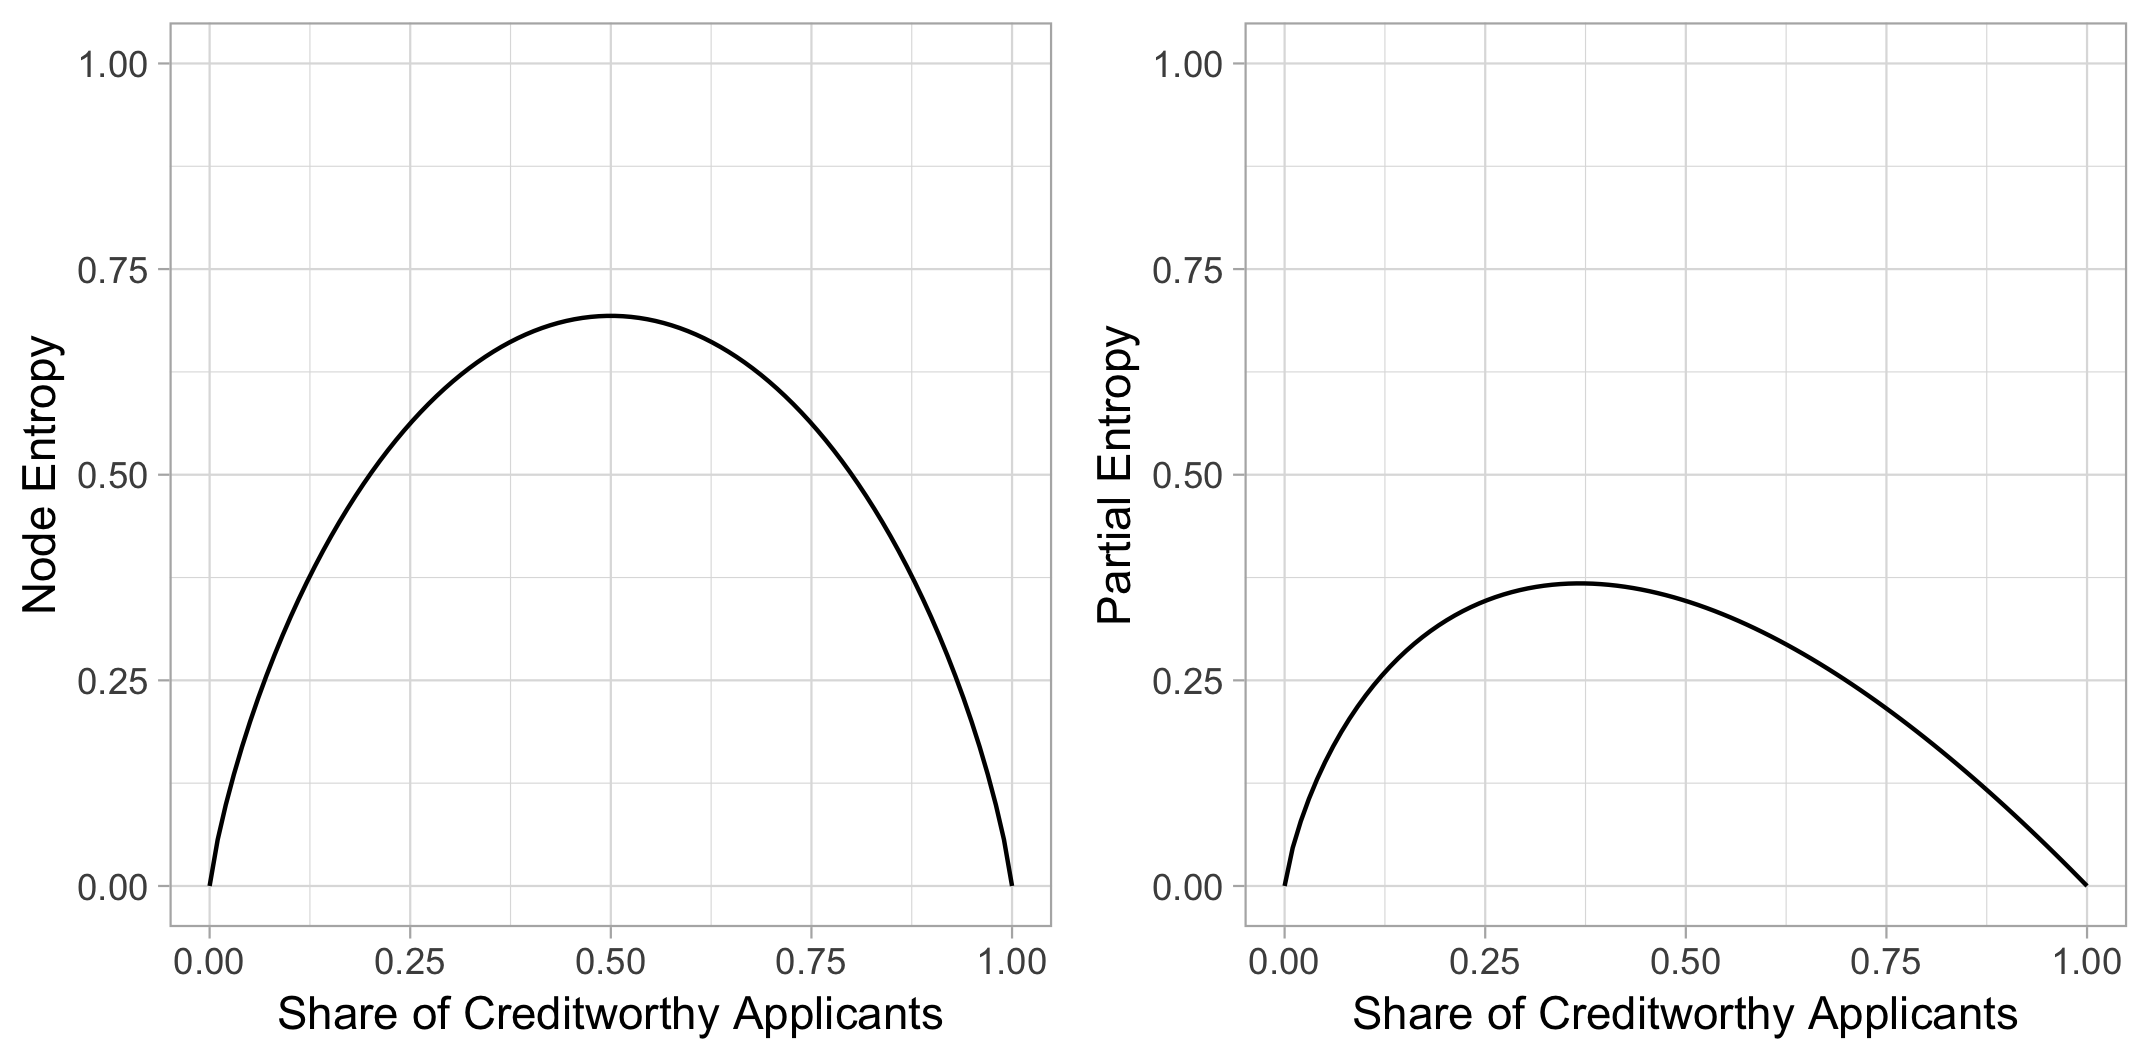
\includegraphics[width=\linewidth]{../content/figs/entropy.png}
  \caption{Entropy}
  \label{fig:entropy}
\end{figure}

% TODO: cite Data Science from Scratch
A popular splitting algorithm is what is called greedy search (\cite{grusDataScienceScratch2015}). It goes as follows: starting from the entire sample as you first node\dots\footnote{This simple version of greedy search could also be complemented with stoping rules related to the depth of the tree and the number of observations in each node. An example of the first case would be: stop when a branch of the tree is made by more than 5 rules, stop. For the second case: stop if the node has less than ten observations in it.}

\begin{itemize}
    \item If the data in the node have all the same label (either creditworthy or defaulting), stop.
    \item Otherwise, try partitioning the applicants by each of the attributes (age, gender, etc).
    \item Choose the splitting rule that results in two new nodes with the lowest entropy weighted by the number of applicants in each node. 
    \item Recur on each newly created node.
\end{itemize}

Once your tree is grown – that is, you have a set of sequential rules that puts each observation in a node –, you now can use it for prediction. You just apply the set of rules to an unknown applicant. If she ends up in a node with a majority of defaulting, you classify her as a default. If the node, however, is composed mainly of creditworthy applicants, you grant her a loan.

\subsection{Honest Causal Tree}

It turns out that slightly adjusting the decision tree can make it a powerful tool for identifying heterogeneous causal effects. An honest causal tree is a modified version of a decision tree that comes with the search for causal effects baked in (\cite{wagerEstimationInferenceHeterogeneous2018}, \cite{atheyGeneralizedRandomForests2016}).

\subsubsection{Why causal?}

We call it a causal tree because the tree tries not to minimize the entropy, but rather to maximize the causal effect in each node. As seen in the previous section, a typical decision tree splits the data by finding which pair of variable and value (for example, the variable could be age and the value 25) can most reduce entropy in the nodes if we were to split the node at it. Since we are interested here in treatment effects, we need to adjust this reasoning a little. First, we cannot observe the same individual under the two states (treatment and control). The best we can do is to identify individuals that are similar and compute the average treatment effect among them. In that vein, we might assume that the treatment effect for all individuals belonging to the same leaf of a tree is the same and can be approximated by the difference between the average of those in treatment and the average of those in control \textit{within} that leaf. Thus, while building the tree, we pick the splits (combinations of variable and value) in such a way that the average treatment effect in the resulting nodes is maximized. In this sense are those trees causal: they have the search for causal effects baked in at their very core.

\subsubsection{Why honest?}

There is another peculiarity of the algorithm used to build causal trees worth mentioning and it's also the reason why they are called honest. The data used to 1) construct the set of rules that specifies the nodes and to 2) estimate the treatment effect of each node are different. In fact, the first step of the causal tree algorithm is to split the training data into two: a \textit{splitting} sample and an \textit{estimation} sample. The tree is then grown on the splitting sample only without ever having access to the estimation sample. Once the tree is fully grown, it's now time to estimate the treatment effect for every leaf in the tree. For that, the estimation sample comes into play and all observations in it are passed through the tree ending up in their respective leaf. Finally, the predicted treatment effect of each leaf of the tree is set to be the difference between the average of individuals in treatment and the average of individuals in control across all the observations (remember, coming from the estimation sample only) that ended up in that leaf.

\subsubsection{From trees to the forest}

As mentioned before, decision trees are very flexible and can accommodate an arbitrarily large amount of rules. Remember: decision trees can be as deep as having one node for each observation in the training set. You wouldn't expect such a tree to generalize to new data. % TODO: cite Business Data Science
As a nonparametric method, it will likely lead to overfitting (as in the case of one node per observation) unless it is regularized. For decision trees, regularization usually takes the form of bagging (\cite{breimanHeuristicsInstabilityStabilization1996}): multiple subsamples from the data are created, the model being regularized is trained on them, and the resulting multiple models have their predictions averaged out into one single model.

A random forest is an example of bagging methods. It is a collection of multiple decision trees that together deliver a single prediction. Each tree of a random forest is trained in a slightly different version of the data. Trees are constructed on random subsamples of both observations and features. The number of observations and the number of features that go in each subsample is the model's hyperparameters, i.e. they must be chosen by the researcher before the random forest is trained. After the random forest is trained and it's supposed to deliver predictions on new data, each tree of the random forest predicts on the new observations and the average of those predictions is the general prediction of the random forest.

This procedure has the benefit of preventing overfitting, a technical term that means your model won't generalize to new data because it is fitting noise (randomness) in the training data. Most importantly, however, for causal forests (a random forest built out of causal trees), \cite{atheyGeneralizedRandomForests2016} have derived that the estimated treatment effects are asymptotically normal. This means that when your sample size gets larger, the distribution of the treatment effect estimates for every end node of our tree approximates the normal distribution. It's then possible to build confidence intervals around those estimates and assess the inherent uncertainty stemming from them.

\newpage

\section{OHIE \& Causal Forests}

Having solidified our understanding of the mechanics of causal forests, we are now ready to apply them to the Oregon Health Insurance Experiment (OHIE) data. \cite{taubmanMedicaidIncreasesEmergencyDepartment2014} have estimated the average treatment effect of Medicaid on emergency department visits to be 0.408 with a p-value lower than 0.001. This result is, therefore, statistically significant and it means that a person under Medicaid is expected to have 0.408 more visits to the emergency department  than what she would have had with no insurance. We have reproduced this result at \url{https://github.com/denismaciel/causal-forest-ohie/tree/master/compiled_analysis/2SLS}. With causal forest, however, we will output one treatment effect estimate per person and by doing that, try to capture the eventual heterogeneity in the data.

\subsection{Variable Selection}

The datasets of OHIE combined have more than 200 variables. This is a high number of dimensions to analyze and is probably well beyond any researcher's ability to consider every possible interaction between those variables\footnote{If we allow for a causal tree to be constructed with only 2 variables, there $40,000 (200 \times 200)$ different trees one could build} and how these interactions might affect the number of visits a person would have with and without Medicaid. 

Here we will consider only 40 out of the over 200 different variables. An exhaustive list of the variables used to train our causal forest can be found in Table \ref{tab:features} in the Appendix. We have removed all variables that were collected \textit{after} the lottery. The reason for that is that policymaking is one of the relevant areas causal forests can potentially be applied to. To include information that only became available after the treatment has been applied would prevent the results from being used in many policy applications, since the policy decision itself is often about to whom treatment should be applied and (for obvious reasons) one doesn't have access to data collected after the application of the treatment at the time such a decision is made.

We have also excluded variables whose meaning not clear from the data dictionaries provided by the authors of the original study. For example, there are some variables related to previous participation in other welfare programs offered by the state of Orgeon. Although these variables might as well improve our causal models, it adds a bit of overhead to the reader and to the analysis itself. For that, we opted to leave them out. %TODO: Should I keep the following reference?
%A detailed overview of which variable was either excluded or kept in the analysis can be found at \href{https:://github.com/denismaciel/causal-forest-ohie/compiled_analysis/causal_forest/}{\texttt{causal\textunderscore forest}}

\subsection{Modeling \& Code}

Before modeling, we have randomly split the data into a train and a test set. The train set contained 80\% of the observations (19,674) while the test set contained the remaining 20\% (4,918). We wanted to have an as close as possible overview of how the model would predict the causal effect for new, completely unseen data. Even though the splitting-estimation-sample procedure, which is already embedded in the causal tree algorithm, ensures that not the same data is used to grow the tree and to estimate the causal effects in the nodes, we go a step further and set aside 20\% of the data, which will remain completely unseen by our causal forest. By doing so, we hope to have a better understanding of how the model will perform on out-of-sample data, which, again, is very important for public policy.

For the modeling itself, we used the \texttt{grf} R package\footnote{The package is open-source and can be found at \url{https://github.com/grf-labs/grf}.}, which is maintained by the authors of the Generalized Random Forest paper. We have used the \texttt{instrumental\textunderscore forest}, which is a generalization of \texttt{causal\textunderscore forest} that accept an instrument together with the independent variables, the treatment and the dependent variable. The causal forest was composed of 2,000 trees. This is the number of trees recommended by the authors if you wish to also estimate confidence intervals along with the treatment effects.

\subsection{Results}

After training the causal forest, we use it to predict the causal effect of Medicaid on the number of visits to the emergency department on the observations in the test set. Figure \ref{fig:rank} shows the estimated causal effects for every observation in the test set ranked by the size.

\begin{figure}
    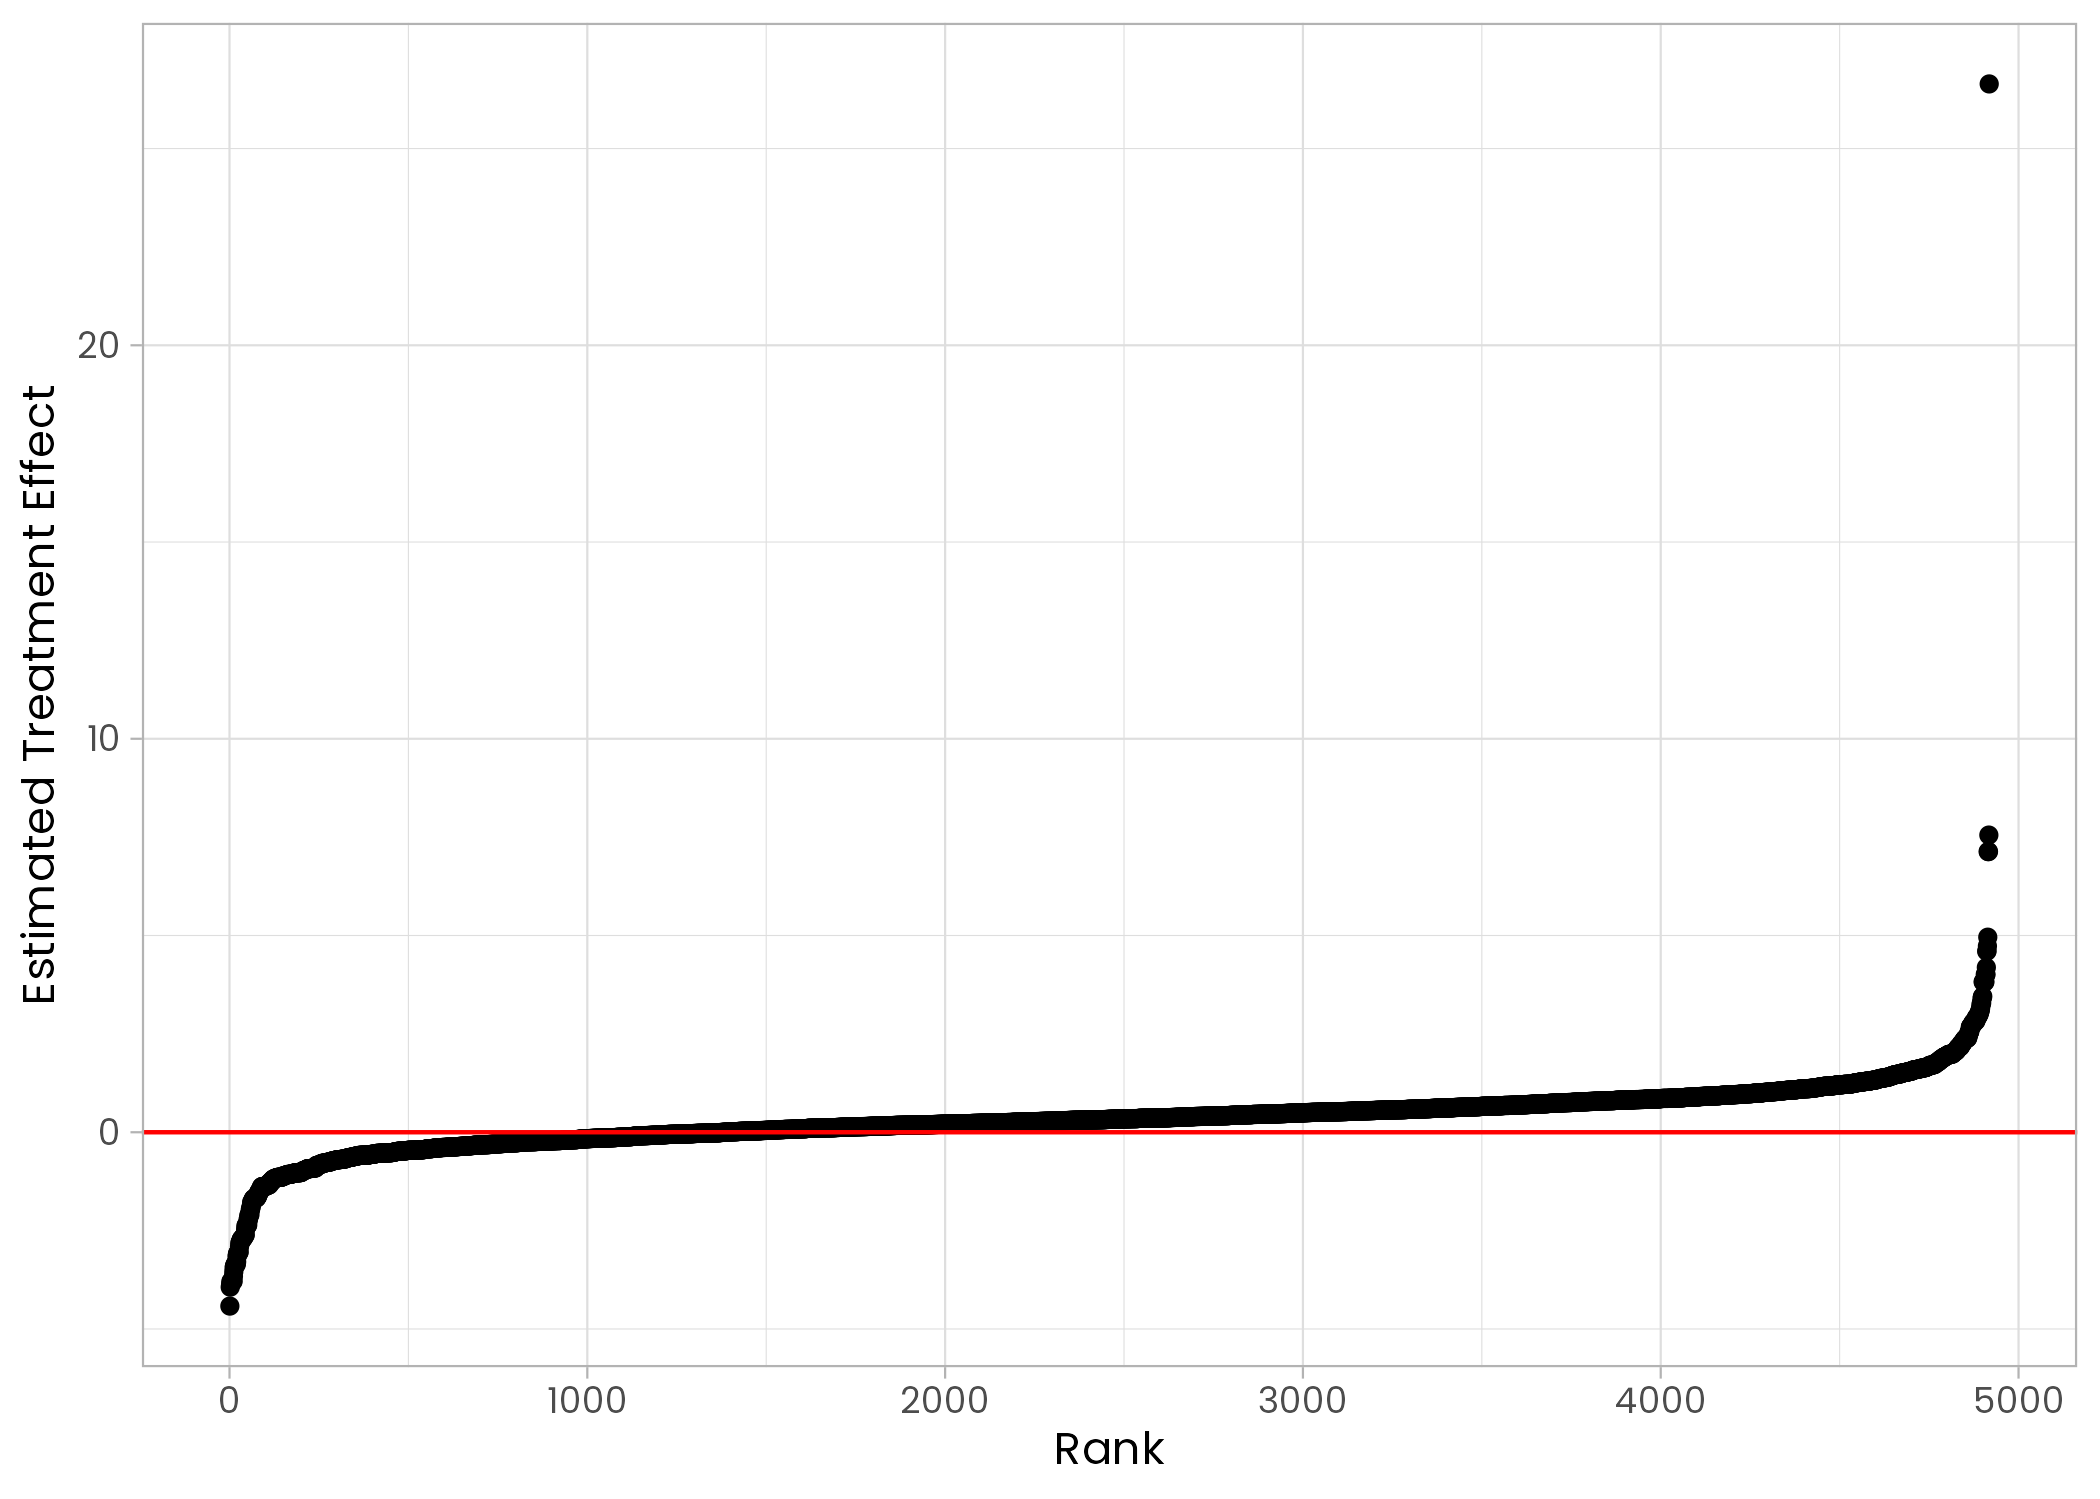
\includegraphics[width=\linewidth]{../content/figs/ete_p_rank.png}
  \caption{Ranked Treatment Effects}
  \label{fig:rank}
\end{figure}

The estimated individual causal effects range from -4.8 to 4.9 with two extreme outliers at -9.8 and 5.4. Compared to the average treatment effect estimate of the original paper (0.408), it seems to indicate that there might be in fact heterogeneity in the effects and that enrollment in Medicaid could increase emergency department visits for some people and decrease it for other people.

Here we are visualizing almost 5 thousand data points and it's difficult to identify where the majority of the observations concentrate: are there more people with negative or positive treatment effects? Figure \ref{fig:histogram} answer this question by making clear that most of the predictions concentrate on the right side of the line of real numbers. This is in line with the original findings and is indicative that Medicaid leads to an increase in emergency department usage for most people.

\begin{figure}
    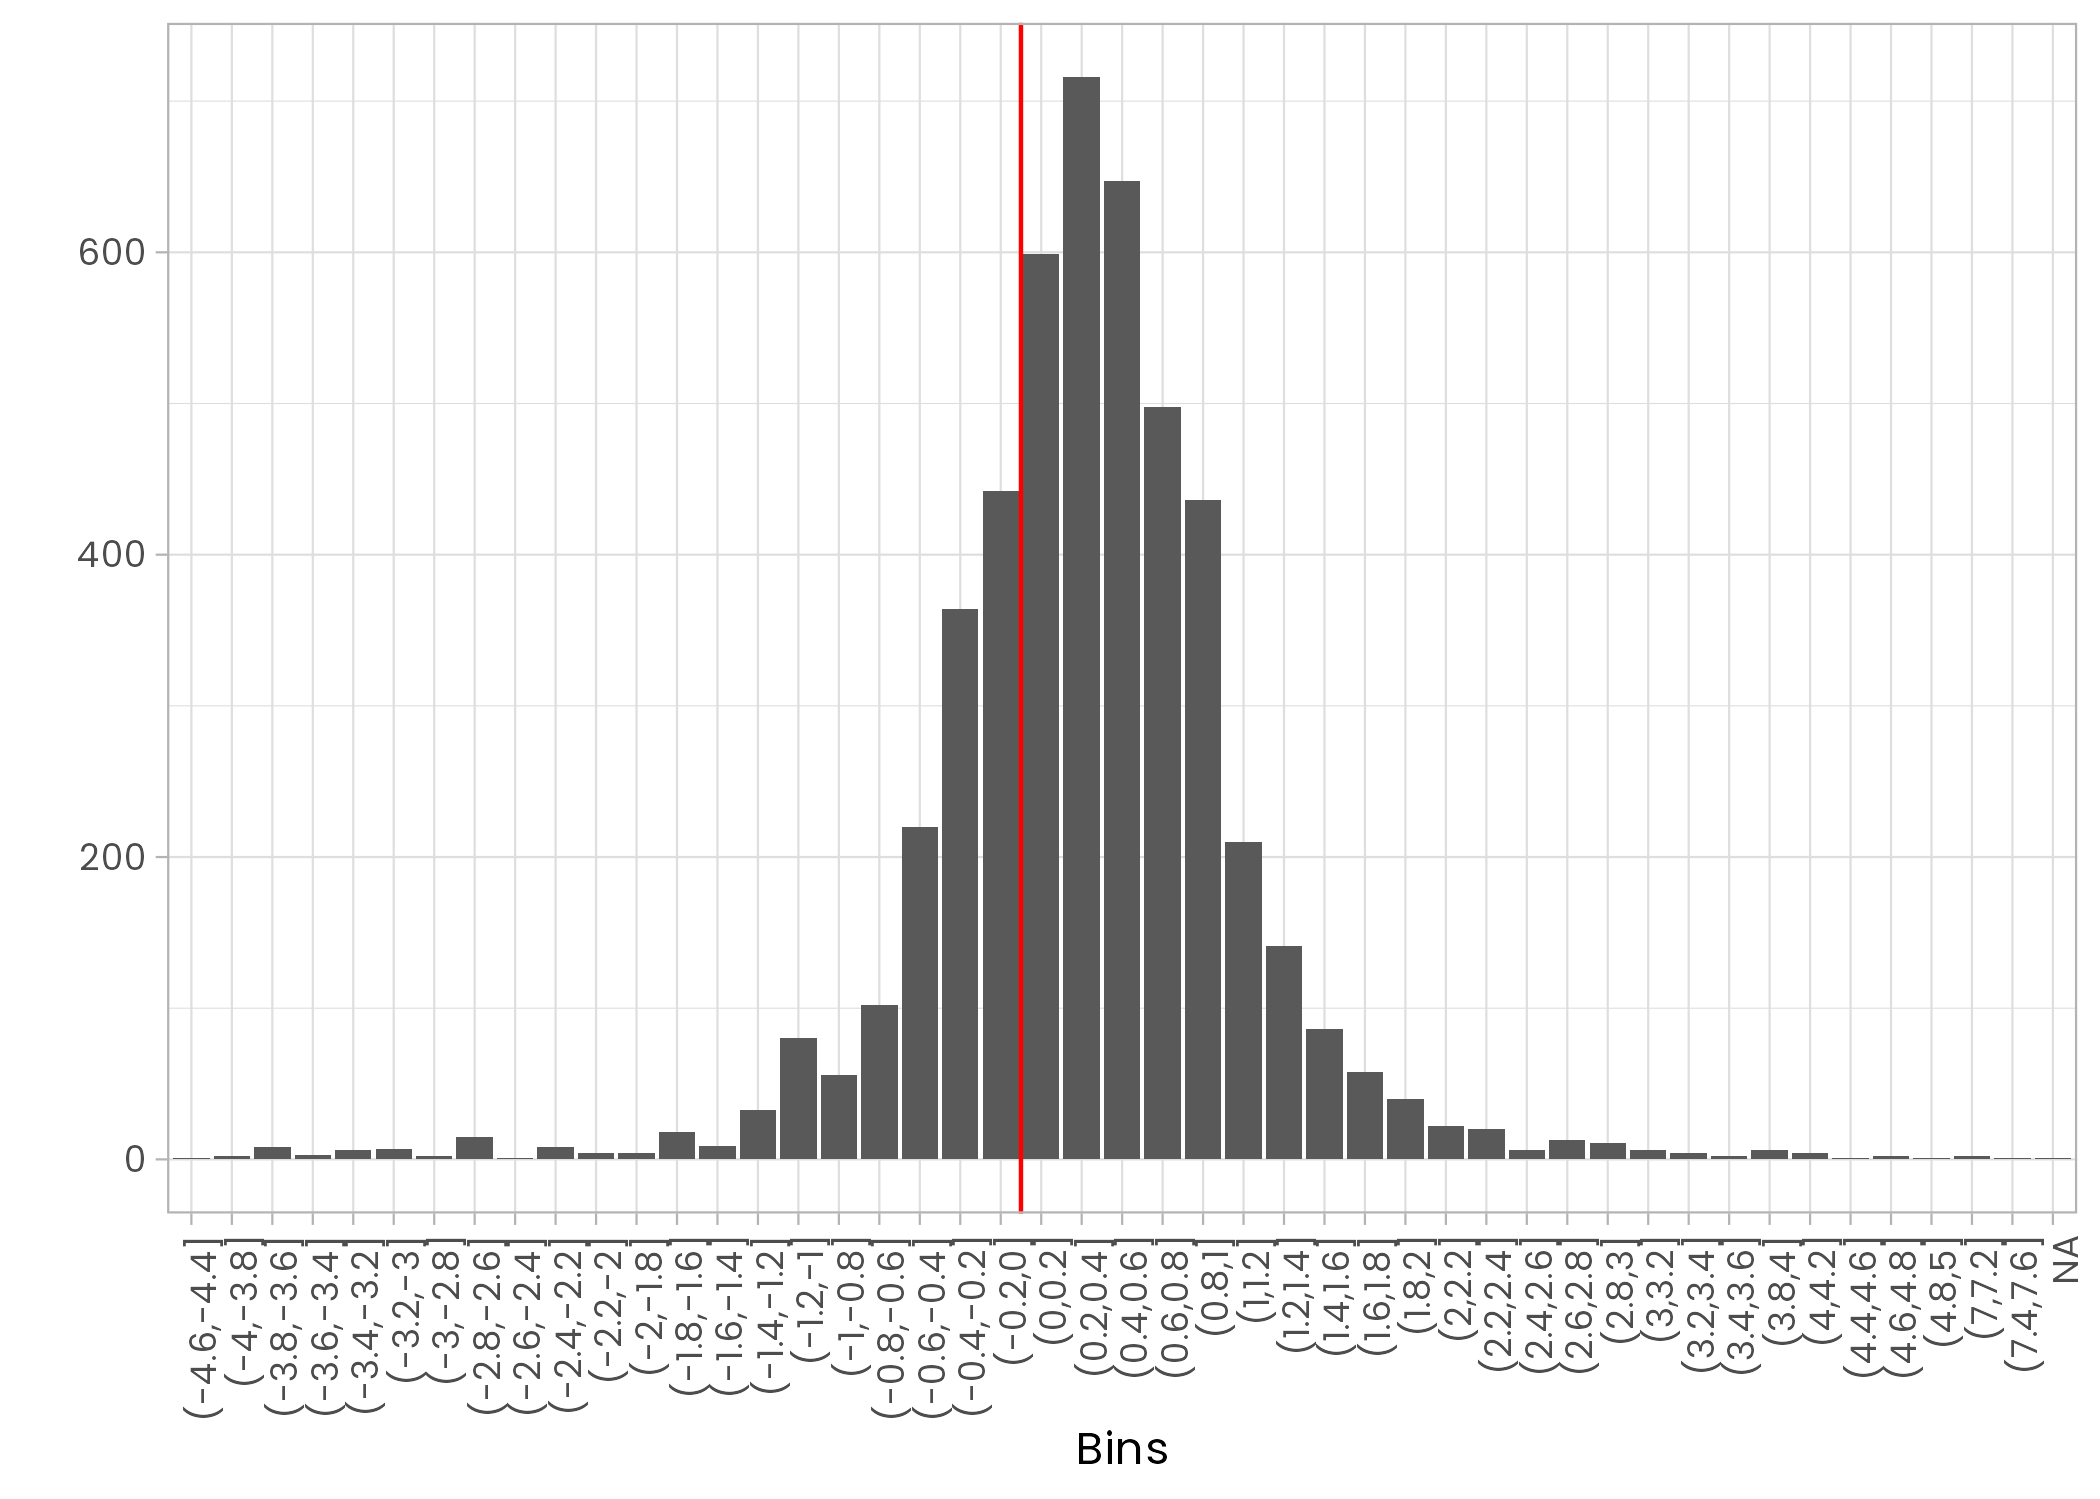
\includegraphics[width=\linewidth]{../content/figs/ete_histogram.png}
  \caption{Treatment Effect Histogram}
  \label{fig:histogram}
\end{figure}

As mentioned, one of the greatest features of causal forests is not only to provide estimates on the heterogeneity of treatment effect but also that these estimates are asymptotically normally distributed. Armed with that, we can construct confidence intervals around our point estimates. In Figure \ref{fig:rank_interval}, we have sampled 200 observations from the test set and displayed the predicted treatment effect estimates accompanied by their respective confidence intervals. There is a great amount of uncertainty on the estimates: even for the highest positive estimates, we cannot reject the null hypothesis with 95\% confidence that they are greater than zero.

\begin{figure}
    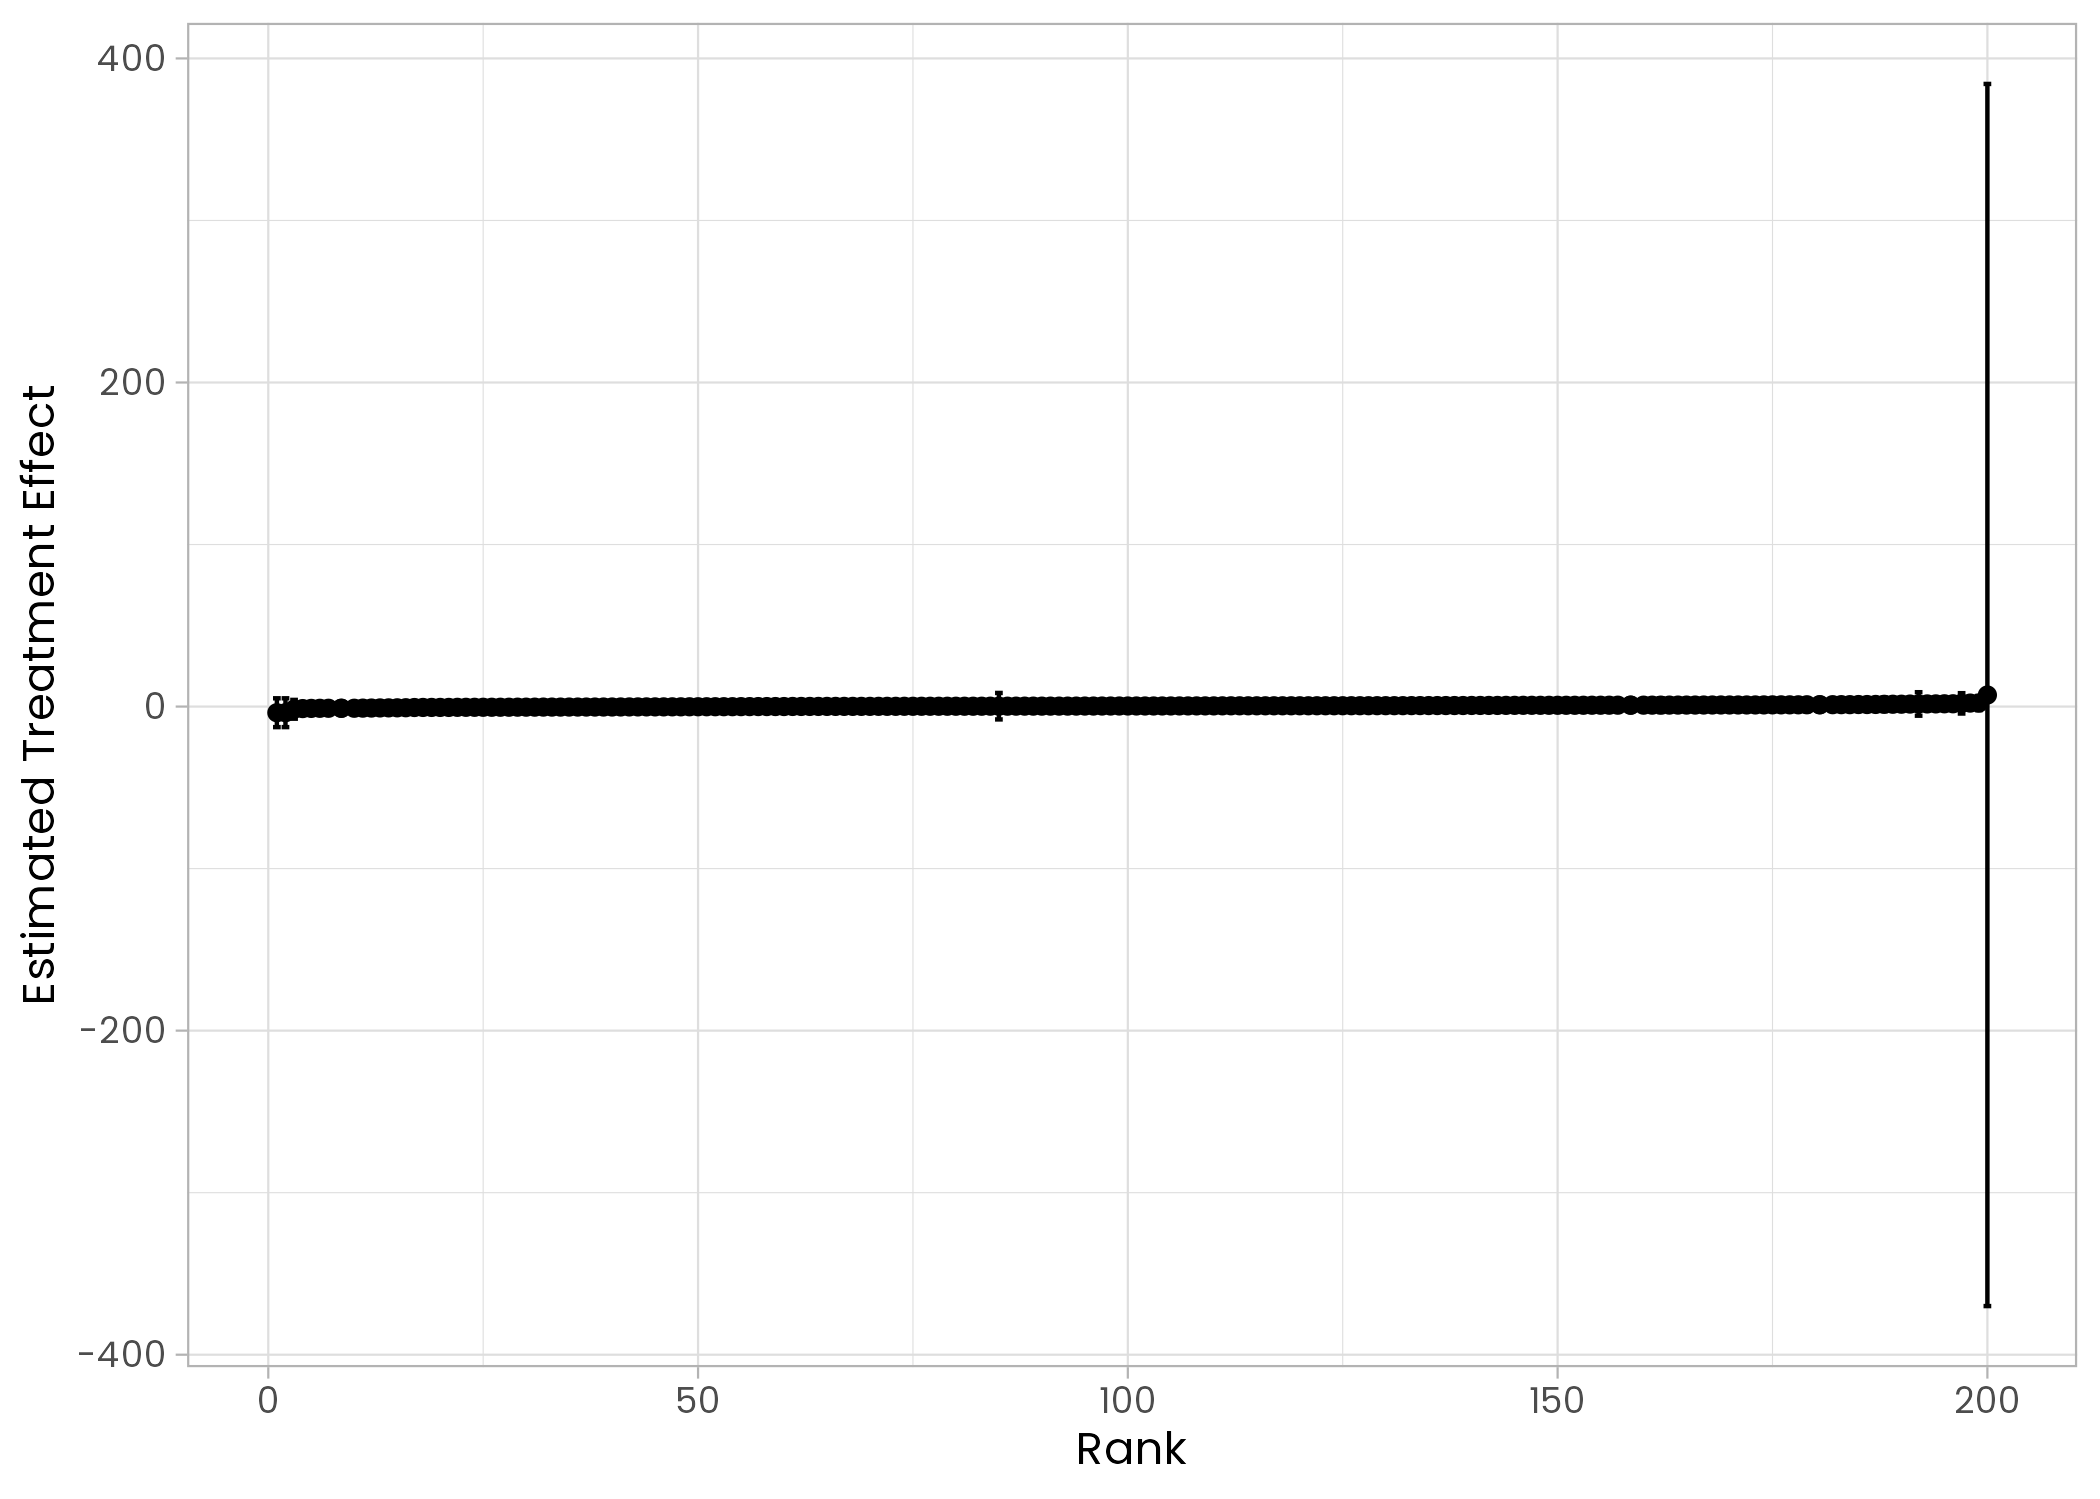
\includegraphics[width=\linewidth]{../content/figs/ete_p_rank_interval.png}
  \caption{Estimated Treatment Effects \& Confidence Intervals}
  \label{fig:rank_interval}
\end{figure}

\subsection{Feature Importance}

Although many machine learning models are known for being difficult to interpret (black box models),\footnote{There have been many efforts lately to make understandable the inner workings of machine learning models. For a good (and free) overview of the techniques on how to interpret these models, see \cite{molnarInterpretableMachineLearning2019}.} feature importance is an interesting metric that allows us to identify which variables are the most relevant for random forests when making decisions.

With so many variables been fed into the causal forest, it is fairly unlikely that all independent variables are equally relevant for estimating causal effects. The feature importance metric assigns to each independent variable a numeric value that represents how relevant it is for the random forest when making its predictions (\cite{hastieElementsStatisticalLearning2009}). Feature importance is calculated according to the following description:

\begin{itemize}
  \item For each node of every tree in the causal forest, determine the variable that splits it. 
  \item For each independent variable, sum up the resulting improvement in the loss function (here: the increase in the difference between treatment and control related to emergency department usage) whenever this variable is used as the splitting criteria.
  \item Normalize the results in such a way that every feature importance lies between 0 and 1 and their sum equals to 1.
\end{itemize}

Table \ref{tab:feature_importance} shows the feature importance for the ten most relevant variables. The most important variable is ``Number of primary care treatable Emergency Department visits'' with 16.66\%. This type of visits encompasses the conditions that require immediate care but could have been treated in a primary care setting. The second and third most important variables are ``Sum of total charges'' and ``Sum of total Emergency Department charges'', which are the amount expended with hospitals in general and with emergency department only, respectively. Except for ``Age in 2009'', all the eight most important variables are related to previous visits to emergency department. Feature importance, however, does not tell us how each feature affects the number of emergency department visits. 

\begin{table}[!ht]
  \centering
  \begin{tabular}{rll}
    \hline
   & Feature & Importance \\ 
    \hline
    1 & num\_epct\_pre\_ed & 16.66\% \\ 
    2 & charg\_tot\_pre\_ed & 14.87\% \\ 
    3 & ed\_charg\_tot\_pre\_ed & 14.51\% \\ 
    4 & num\_edcnnp\_pre\_ed & 10.89\% \\ 
    5 & num\_ne\_pre\_ed & 10.81\% \\ 
    6 & num\_edcnpa\_pre\_ed & 7.08\% \\ 
    7 & age\_2009 & 4.31\% \\ 
    8 & num\_unclas\_pre\_ed & 2.58\% \\ 
    9 & any\_hosp\_pre\_ed\_Yes & 2.46\% \\ 
    10 & any\_chron\_pre\_ed\_Yes & 2.44\% \\ 
     \hline
  \end{tabular}
  
  \caption{\label{tab:feature_importance} Feature importance of most important variables}
  \end{table}

\newpage

\section{Final Remarks}

After a brief tour on topics such as causality, heterogeneity in treatment effects and decision trees, we managed to apply a causal forest to real-world data. Causal forest is a promising method to uncover heterogeneity in causal effects, specially for large datasets. It applies battle-tested principles developed in machine learning to causal analysis and it has also convenient statistical properties that allow us to assess the certainty of its estimates. For the Oregon Health Insurance Experiment, causal forests seemed to have identified large differences across its participants with respect to the response to Medicaid coverage. However, the uncertainty of the estimates are very high, which does not allow us to neither confirm the existence nor exclude the possibility of heterogeneous treatment effects.

% ----------------
% --- appendix ---
% ----------------

\input{../content/var/appendix}

% --------------------------------------------
% --- last page: Declaration of Authorship ---
% --------------------------------------------

% \newpage
% \thispagestyle{empty}
% \input{../content/fix/authorship}

\end{document}

